\documentclass[10pt]{article}

% --------- Fonts and colors -----------------------------
% This way can use any TrueType font on Mac with XeLaTeX
\usepackage{fontspec}
\setmainfont{Helvetica}
%\setromanfont{Times New Roman}
\setsansfont{Helvetica}
%\setmonofont{Courier}

\usepackage{underscore} % not sure if needed for underscores in identifiers
\usepackage{marvosym} % for lightning symbol

% ---------- Layout ---------------------------------------
\setlength{\parindent}{0pt}
\setlength{\parskip}{1em}

% for externally generated figures
\usepackage[xetex]{graphicx}

% ---------- Fancy versions of basic things ---------------
\usepackage{alltt,xcolor} % use color in verbatim-like environment alltt

\usepackage{amsmath}

\usepackage{bytefield} % For memory layout

\usepackage{float} % To place figures exactly where we want them

% ---------- Graphics and figures --------------------------
%\usepackage{tikz} % For drawing circles around numbers
%\usetikzlibrary{shapes, arrows, positioning}


% Comment out blocks easily
\newcommand\comment[1]{}

\newcommand\figurebreak{}

%\renewcommand\figurebreak{\pagebreak}  % uncomment to place each LaTeX figure on its own page (not for imported PDF figures)

%\pagenumbering{gobble} % uncomment to hide page numbers

\title{\vskip -1.2in {GT-Pro Query Engine} \vskip -0.5in}
\date{}

\newcommand\AllelesTable{\textbf{Alleles \hbox{Table}}}
\newcommand\KmersTable{\textbf{Kmers \hbox{Table}}}

\begin{document}
\maketitle

\tableofcontents

% A palette of bytefields

\section{Database Size Reduction}


GT-Pro's gut genome database consists of 2.8 billion kmers that cover 52.8 million bi-allelic SNPs across 881 species.  Each kmer is 31 base pairs long and occurs in a unique species.

GT-Pro uses 4 bytes to represent each kmer and 48 bytes to represent each SNP, for a total of 13 GB -- twice as compact compared to bzip2 compression.
\begin{itemize}
\item The database download takes less time.
\item Queries run at full speed immediately after download.
\item Parallel runs share the database in RAM via memory mapping.
\end{itemize}

To accelerate queries, GTPro uses an index and a bloom filter for the kmers present in the database.  These auxiliary data structures may be downloaded with the database or built locally from it.

In AWS, all required downloads -- of the database, index, and bloom filter -- complete in 30 seconds or less.  With slower networking, one has the option to download just the database, then build the index and bloom filter locally.

For faster download speeds in AWS, we recommend using an instance with at least 10 Gbps networking, and following the instructions in \\ \texttt{https://github.com/chanzuckerberg/s3mi}.

\pagebreak

\subsection{Kmers Table}


The database consists of two tables.
\begin{itemize}
\item A 10.6 GB table containing a 4-byte entry for each kmer.
\item A 2.4 GB table containing a 24-byte entry for each allele.
\end{itemize}
\figurebreak
\vskip 1em
\begin{bytefield}[bitwidth=0.9em, bitheight=4em]{32}

 \bitheader{0-31} \\
 
 \begin{leftwordgroup}{\parbox{3.5em}{\small\raggedright 2.86\\ billion\\kmers \\ \vskip 1em \textbf{Colex}\\ \textbf{order} \\ on nt. \\ seq.}}

 \bitbox{5}{\small{snp_offset}} & \bitbox{27}{\small{allele_index}}\\
 
 \bitbox{5}{\small{snp_offset}} & \bitbox{27}{\small{allele_index}} \\
 
 \wordbox[lrt]{1}{\vskip 1.9em 2,856,121,626 rows \\
                  \vskip 0.5em 10.64 GB total \\ } \\
 
 \skippedwords \\
 
 \wordbox[lrb]{1}{} \\

 \bitbox{5}{\small{snp_offset}} & \bitbox{27}{\small{allele_index}}
 
\end{leftwordgroup}
 
\end{bytefield}
\figurebreak
\vskip 1em

Each entry in the \KmersTable{} is comprised of a 5 bit \textit{snp_offset} and 27 bit \textit{allele_index} that together represent a kmer.

The \textit{snp_offset} identifies the SNP position within the kmer.  It's the count of nucleotides in the kmer that precede the SNP, a number between 0 and 30.

The \textit{allele_index} points to an entry in the \AllelesTable{} from which the kmer's entire sequence can be recovered through the formula
$$
\hbox{\textit{kmer_seq}} := \hbox{substr}(\hbox{\textit{allele_seq}}, \,30 - \hbox{\textit{snp_offset}}, \,31)
$$
See subsection "Overlap Encoding" below.
\pagebreak

\subsection{Overlap Encoding}


The major and minor allele of a SNP may each be covered by up to 31 different kmers, with \textsl{snp_offset} values 0, 1, $\ldots$ 30.  Some kmers would be absent from the database because they bear too little information about their origin (for instance, kmers that occur in multiple species).

In the illustration below, only 6 of the possible 31 kmers are present for the major allele, and 5 for the minor allele.  There are two distinct kmers with \textsl{\hbox{snp_offset = 10}}.  The first of those covers \textsl{allele_seq_major} and the second covers \textsl{allele_seq_minor}.
\newcommand\snp[1]{\textcolor{orange}{\fbox{\textbf{#1}}}}
\newcommand\snpp[1]{\textcolor{brown}{\fbox{\textbf{#1}}}}

\figurebreak
\hbox{\vbox{
\begin{alltt}
\small
                              \snp{SNP}                           snp_offset

 \rule[1em]{37em}{0.4pt}
 ..............................\snp{G}GTCTAGGCGCAATGTAACGCTTTTATCGCT       0
 ..........................TCTT\snp{G}GTCTAGGCGCAATGTAACGCTTTTAT....       4
 ....................GCTTAGTCTT\snp{G}GTCTAGGCGCAATGTAACGC..........      10'
 ...............TTAGCGCTTAGTCTT\snp{G}GTCTAGGCGCAATGT...............      15
 ............GACTTAGCGCTTAGTCTT\snp{G}GTCTAGGCGCAA..................      18
 .........CTAGACTTAGCGCTTAGTCTT\snp{G}GTCTAGGCG.....................      21
\hspace{0.16em}\textcolor{magenta}{\fbox{CAACTATTCCTAGACTTAGCGCTTAGTCTT\snp{G}GTCTAGGCGCAATGTAACGCTTTTATCGCT}  allele_seq_major}
\hspace{0.16em}\textcolor{magenta}{\fbox{CAACTATTCCTAGACTTAGCGCTTAGTCTT\snpp{C}GTCTAGGCGCAATGTAACGCTTTTATCGCT}  allele_seq_minor}
 ....................GCTTAGTCTT\snpp{C}GTCTAGGCGCAATGTAACGC..........      10"
 ..............CTTAGCGCTTAGTCTT\snpp{C}GTCTAGGCGCAATG................      16
 .........CTAGACTTAGCGCTTAGTCTT\snpp{C}GTCTAGGCG.....................      21
 .....ATTCCTAGACTTAGCGCTTAGTCTT\snpp{C}GTCTA.........................      25
 ....TATTCCTAGACTTAGCGCTTAGTCTT\snpp{C}GTCT..........................      26

\end{alltt}
}}
\figurebreak

Altogether, the 11 kmers above contain 341 base pairs.  Their shared \hbox{\textsl{allele_seq}}'s (major and minor) comprise only 122 base pairs, from which the kmers can be recovered fully.  That's how overlap encoding achieves high compression. 

Each 61-bp \textsl{allele_seq} is stored into a separate entry in the \AllelesTable{}.

\pagebreak


\subsubsection{Multi-SNP Kmers}


If multiple SNPs occur in close proximity, some of the overlapping kmers may not completely agree.  In the illustration below, a lightning symbol indicates the position of a second SNP over which some kmers disagree.
\newcommand\bolt{\textcolor{red}{\Lightning}}

\newcommand\snq[1]{\textcolor{red}{\textbf{#1}}}
\newcommand\snr[1]{\textcolor{blue}{\textbf{#1}}}

\figurebreak

\hbox{\vbox{
\begin{alltt}
\small
              \fbox{\bolt}              \snp{SNP}                           snp_offset

 \rule[1em]{37em}{0.4pt}
 ..............{\bolt}...............\snp{G}GTCTAGGCGCAATGTAACGCTTTTATCGCT       0
 ..............{\bolt}...........TCTT\snp{G}GTCTAGGCGCAATGTAACGCTTTTAT....       4
 ..............{\bolt}.........AGTCTT\snp{G}GTCTAGGCGCAATGTAACGCTTTT......       6
 ............GA\snq{C}TTAGCGCTTAGTCTT\snp{G}GTCTAGGCGCAA..................      18'
\hspace{0.16em}\textcolor{magenta}{\fbox{CAACTATTCCTAGA\snq{C}TTAGCGCTTAGTCTT\snp{G}GTCTAGGCGCAATGTAACGCTTTTATCGCT}  allele_seq_major}
\hspace{0.16em}\textcolor{magenta}{\fbox{CAACTATTCCTAGA\snq{C}TTAGCGCTTAGTCTT\snpp{C}GTCTAGGCGCAATGTAACGCTTTTATCGCT}  allele_seq_minor}
 ............GA\snq{C}TTAGCGCTTAGTCTT\snpp{C}GTCTAGGCGCAA..................      18"
 .........CTAGA\snq{C}TTAGCGCTTAGTCTT\snpp{C}GTCTAGGCG.....................      21
\hspace{0.16em}\textcolor{magenta}{\fbox{CAACTATTCCTAGA\snr{G}TTAGCGCTTAGTCTT\snpp{C}GTCTAGGCGCAATGTAACGCTTTTATCGCT}  allele_seq_minor_2}
 ........CCTAGA\snr{G}TTAGCGCTTAGTCTT\snpp{C}GTCTAGGC......................      22
 ....TATTCCTAGA\snr{G}TTAGCGCTTAGTCTT\snpp{C}GTCT..........................      26

\end{alltt}
}}

\figurebreak

Encoding the discordant kmers in this case requires the introduction of another entry into the \AllelesTable to represent \textsl{allele_seq_minor_2}.  In some cases, up to 11 SNPs have been seen in such close proximity.  Approximately 1.8 percent of allele table entries exist for this purpose.

\subsection{Alleles Table}


\figurebreak

\begin{bytefield}[bitwidth=0.54em]{64}
 \bitheader{0,1,55,61,63} \\
 
 \begin{rightwordgroup}{\footnotesize{allele}\\ \footnotesize{entry}\\ \footnotesize{0}}

 \bitbox{2}{\tiny{XX}} &
 \bitbox{60}{\footnotesize{allele_seq:  30 bp before SNP (60 bits)}} &
 \bitbox{2}{\tiny{SNP}} \\

 \bitbox{2}{\tiny{SNP}} &
 \bitbox{60}{\footnotesize{allele_seq:  30 bp after SNP (60 bits)}} &
 \bitbox{2}{\tiny{XX}} \\
 
 \bitbox{56}{\footnotesize{snp_coord (56 bits)}} &
 \bitbox{8}{\footnotesize{reserved}}
 \end{rightwordgroup}\\ \\
 
 \begin{rightwordgroup}{\footnotesize{allele}\\ \footnotesize{entry}\\ \footnotesize{1}}

 \bitbox{2}{\tiny{XX}} &
 \bitbox{60}{\footnotesize{allele_seq:  30 bp before SNP (60 bits)}} &
 \bitbox{2}{\tiny{SNP}} \\
 
 \bitbox{2}{\tiny{SNP}} &
 \bitbox{60}{\footnotesize{allele_seq:  30 bp after SNP (60 bits)}} &
 \bitbox{2}{\tiny{XX}} \\
 
 \bitbox{56}{\footnotesize{snp_coord (56 bits)}} &
 \bitbox{8}{\footnotesize{reserved}}
 \end{rightwordgroup}\\ \\

 \wordbox[lrt]{4}{\vskip 1em \footnotesize{107,565,805 alleles (1.8\% multi-SNP) \\ \vskip 0.5em for 52.8 million SNPs \\ \vskip 0.5em 3 dwords per allele \\ \vskip 0.5em 2.4 GB total}} \\
 
 \skippedwords \\
 
 \wordbox[lrb]{1}{} \\ \\

 \begin{rightwordgroup}{\footnotesize{allele}\\ \footnotesize{entry}\\ \footnotesize{N -- 1}}

 \bitbox{2}{\tiny{XX}} &
 \bitbox{60}{\footnotesize{allele_seq:  30 bp before SNP (60 bits)}} &
 \bitbox{2}{\tiny{SNP}} \\
 
 \bitbox{2}{\tiny{SNP}} &
 \bitbox{60}{\footnotesize{allele_seq:  30 bp after SNP (60 bits)}} &
 \bitbox{2}{\tiny{XX}} \\
 
 \bitbox{56}{\footnotesize{snp_coord (56 bits)}} &
 \bitbox{8}{\footnotesize{reserved}}
 \end{rightwordgroup}\\ \\

\end{bytefield}

\figurebreak


Each entry in the \AllelesTable{} represents a specific SNP and allele by encoding the 61 nucleotide \hbox{\textit{allele_seq}} centered on the SNP, along with the species id (6 decimal digits), major/minor allele indicator (0 or 1), and genomic coordinate of the SNP.  The allele nucleotide itself, \hbox{\textsl{allele_seq(30)}}, is represented redundantly in dwords 0 and 1.

\pagebreak

\section{Query Acceleration}


\subsection{Index}


For any nucleotide sequence \textsl{S}, the kmers that end with \textsl{S} occupy consecutive rows in the \KmersTable{}.  They can be quickly located with an an index that simply maps \textsl{S} to the range of rows that share \textsl{S}.

For any given 31-bp kmer \textsl{query}, the following algorithm locates every allele in the database that is covered by \textsl{query}.
\begin{itemize}
\item Look up 16-bp suffix of \textsl{query} in \textbf{Index}.
\item If found, examine all \KmersTable{} entries referred by \textbf{Index}.
\item Decode each referred entry through \AllelesTable{} to recover a \textsl{db_kmer} that's a possible match for \textsl{query}.  Compare entire nucleotide sequence of \textsl{db_kmer} to \textsl{query}. If exact match, emit allele info.
\end{itemize}


\subsection{Bloom Filter}
A similar technique helps reject queries with absent prefix.  The set of 18-bit kmer prefixes in the database is encoded as a bit vector and consulted for each query.  We call this a bloom filter.

In more detail, a vector of $\text{2}^\text{36}$ bits is initialized so \hbox{\textsl{bit_vector[bit_address]}} is 1 if and only if interpreting \textsl{bit_address} itself as an 18-bp nucleotide sequence (see next section) yields the prefix of some kmer in the database.

The amended query algorithm is now
\begin{itemize}
\item Look up \textsl{query} prefix in \textbf{Bloom Filter}.
\item If found, look up \textsl{query} suffix in \textbf{Index}.
\item If found, examine all \KmersTable{} entries referred by the index one by one, as before.
\end{itemize}

Why exactly 16 nucleotide suffix and 18 nucleotide prefix?  GT-Pro supports a range of values for these parameters, with defaults that perform best for the available amount of RAM.  See figure "Query Speed vs Memory Footprint".


\pagebreak

\subsection{Integer Encoding}


In binary encoding each nucleotide takes 2 bits.

Nucleotide strings are encoded so that their initial characters map to lower memory addresses / less significant bits.

A common trick is to interpret a nucleotide sequence as an integer, use that integer as an array index, or sort those integers to create a substrate for efficient sequence lookups.

The following table illustrates how integer sort order on the encodings corresponds to \textbf{colex order} on the original nucleotide strings.

\figurebreak

\hbox{\vbox{
\begin{alltt}
Nucleotide    Binary Encoding         Integer
Sequence      (LSB {\ldots} MSB)               Value
\rule[0.2em]{24em}{0.4pt}
AACGCCA\ldots      00001001101000\ldots           1,424
AACGCGA\ldots      00001001100100\ldots           2,448
AACGTGA\ldots      00001001110100\ldots           2,960
AACGAGT\ldots      00001001000111\ldots          14,480
AACGCGT\ldots      00001001100111\ldots          14,736
\end{alltt}
}}

\figurebreak

When constructing the index and bloom filter we may use odd numbers of bits from these integer encodings in order to fine-tune memory use (see parameters \texttt{-l} and \texttt{-m} in figure "Query Speed vs Memory Footprint").

\pagebreak

\subsection{Representing the Index with an Array}


Conceptually, the index is a map from nucleotide strings -- all possible kmer suffixes -- to row ranges in the \KmersTable{}.  Constraining the domain of the map to suffixes of a specific length -- usually up to 16 nucleotides -- makes the RAM requirements acceptable.

As the database contains 2.8 billion kmers, the 16-bp domain of this map (with 4.3 billion possible suffixes) is densely covered.  Therefore, a simple linear array is better-suited to represent this map than, say, a hash table.

Each entry of the \textbf{Index Array} is comprised of a 48-bit \textsl{range_start} and 16-bit \textsl{range_length} representing a range of rows in the \KmersTable{} that all share the same suffix.

To lookup a suffix string \textsl{S}, first encode \textsl{S} as an integer \textsl{I}, then find element \textsl{I} in the \textbf{Index Array}.  If that element is zero, the suffix does not occur in the database. Otherwise, the element's \textsl{range_start} and \textsl{range_length} tell you which \KmersTable{} rows to examine.

\figurebreak

\vskip 1em
\begin{bytefield}[bitwidth=0.5em]{64}
 \bitheader{0,47,63}\\
 
 \begin{rightwordgroup}{\texttt{AAA{\ldots}AA}}
 \bitbox{48}{\footnotesize range_start} & \bitbox{16}{\footnotesize range_length}
 \end{rightwordgroup}\\
 
 \begin{rightwordgroup}{\texttt{CAA{\ldots}AA}}
 \bitbox{48}{\footnotesize range_start} & \bitbox{16}{\footnotesize range_length}
 \end{rightwordgroup}\\
 
 \begin{rightwordgroup}{\texttt{GAA{\ldots}AA}}
 \bitbox{48}{\footnotesize range_start} & \bitbox{16}{\footnotesize range_length}
 \end{rightwordgroup}\\
 
 \wordbox[lrt]{2}{\footnotesize\vskip 1.9em 4,294,967,296 rows \\
                  \footnotesize\vskip 0.5em 32 GB total \\ } \\
 
 \skippedwords \\
 
 \wordbox[lrb]{1}{} \\

 \begin{rightwordgroup}{\texttt{TTT{\ldots}TT}}
 \bitbox{48}{\footnotesize range_start} & \bitbox{16}{\footnotesize range_length}
 \end{rightwordgroup}\\
 
\end{bytefield}

\figurebreak

The suffix length and size of the index array are configurable,
with defaults that maximize performance for the available RAM.


\section{Performance and Scalability Measurements}


All measurements reflect full utilization of all cores on the respective machines over most of the execution time.
Execution is never I/O bound.

\figurebreak

\renewcommand{\arraystretch}{2.0}
\begin{center}
\footnotesize
\begin{tabular}{|c|c|c|c|c|r|r|}
\hline
Method & Environment & CPU cores & RAM & Samples & \,\,\,\,Reads$^\dagger$\,\,\,\, & Reads\,/\,sec
\\ \hline
Bowtie+Pileup & Server & 24 & 384 GB & 36 & 173 million & 18,036\phantom{*}
\\ \hline
GT-Pro                & Server & 24 & 384 GB & 24 &  72 million & 999,158*
\\ \hline
GT-Pro                & Laptop & 8 & 32 GB & 16 &  24 million & 212,203*
\\ \hline
\end{tabular}

$^\dagger$Average read length is 148 base pairs after QC.\vphantom{\huge y}
\\
\vphantom{\Huge y}$^*$ Each GT-Pro measurement is the average of 8 repetitions.
\end{center}
\figurebreak



\subsection{Baseline Reference}


We compared the performance of GT-Pro to a method that produces equivalent results using read alignment and pile-up counting.

The method runs bowtie first, which can align 61,401 reads per second on our 24-core server.

Then it runs pileup with PySAM at 25,528 reads per second utilizing all 24 cores.

This yields 18,036 reads per second, which is 55.4 times slower than GT-Pro on the same machine.

\subsection{Sample Selection}


Performance was measured on nucleotide sequences from SRA study SRP110665, human gut microbiome fecal samples from Hadza hunter-gatherers in Tanzania, available at \,\,\texttt{https://www.ncbi.nlm.nih.gov/Traces/study/?acc=SRP110665.}

The selection of samples and reads is arbitrary.  For bowtie and pileup, the chosen 36 samples were processed in their entirety.  For GT-Pro laptop, each sample contributed just its first 1.5 million reads.  For GT-Pro server, the first and the last 1.5 million reads were used.

\subsection{Reducing Variance in the Compute Environment}


Great care was taken to obtain reliable and consistent performance measurements from run to run.   In the server environment, this involved choosing a machine with a single NUMA node,
using the \texttt{taskset} utility to ensure each CPU core runs the same number of threads, and disabling the Linux memory defragmenter via
\begin{alltt}
    echo never > /sys/kernel/mm/transparent_hugepage/defrag
\end{alltt}

The effectiveness of these measures is evident in figure "Query Speed vs Memory Footprint", where the 8 distinct measurements for every server configuration overlap closely.  We did not control these system parameters on the MacBook Pro laptop, and the same figure reflects noticeable variance in the laptop data. 

The reduced variance in server performance enables us to iterate efficiently even on minor algorithmic improvements.  It also allows us to sweep across a large number of possible choices for the index and bloom filter sizes, characterizing the optimal configuration as a function of available RAM.

Users of GT-Pro do not need to tweak their Linux settings to achieve peak performance.  In fact, a freshly booted Linux system without any tweaks should register even higher performance.  However, that performance will tend to degrade and vary over time.  Our tweaks ensure it remains consistent for benchmarking.

We ran all server tests, including Bowtie + Pileup, under the same conditions.

We used \texttt{sar} and \texttt{htop} to monitor CPU and I/O utilization during server runs.

No tweaks were applied to the laptop environment.

\pagebreak
\subsection{Multicore Performance}


\hskip-3.5em\makebox[0pt][l]{
  \raisebox{-\totalheight-6em}[0pt][0pt]{
      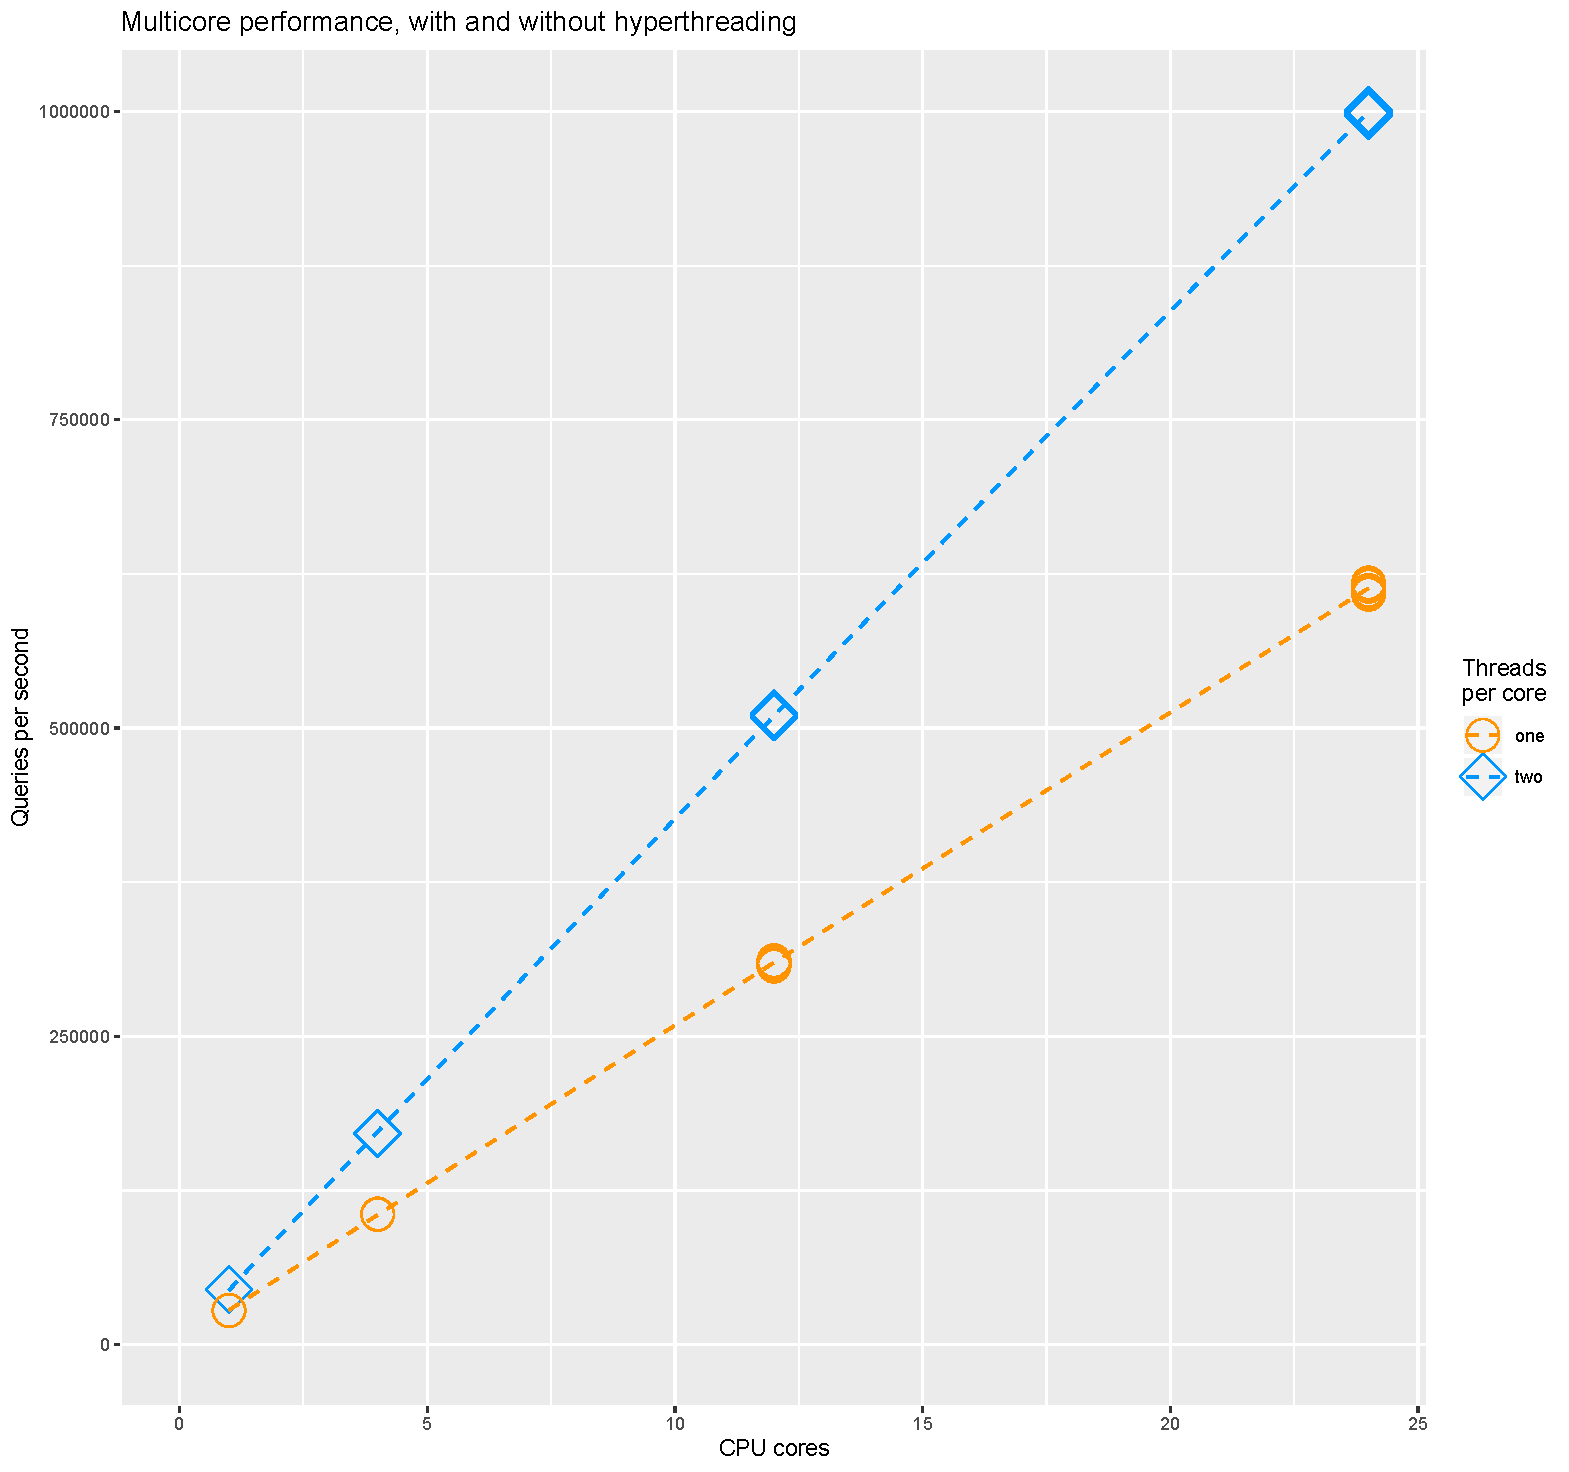
\includegraphics[width=1.2\textwidth]{multiperf.pdf}
  }
}
\vskip -0.4in

We varied the number of CPU cores while controlling the number of threads per core using the Linux \texttt{taskset} utility.  Each config ran 8 times.

System performance scaled linearly with the number of cores and was higher with hyperthreading.


\pagebreak
\subsection{Multicore Efficiency}


\hskip-3em\makebox[0pt][l]{
  \raisebox{-\totalheight-6em}[0pt][0pt]{
      \includegraphics[width=1.15\textwidth]{multieff.pdf}
  }
}
\vskip -0.4in

We varied the number of CPU cores while controlling the number of threads per core using the Linux \texttt{taskset} utility.  Each config ran 8 times.

Per-core performance remained relatively constant, and was higher with hyperthreading.



\pagebreak
\subsection{Server Parameter Sweeps}


\hskip-0.7in\makebox[0pt][l]{
  \raisebox{-\totalheight-7em}[0pt][0pt]{
      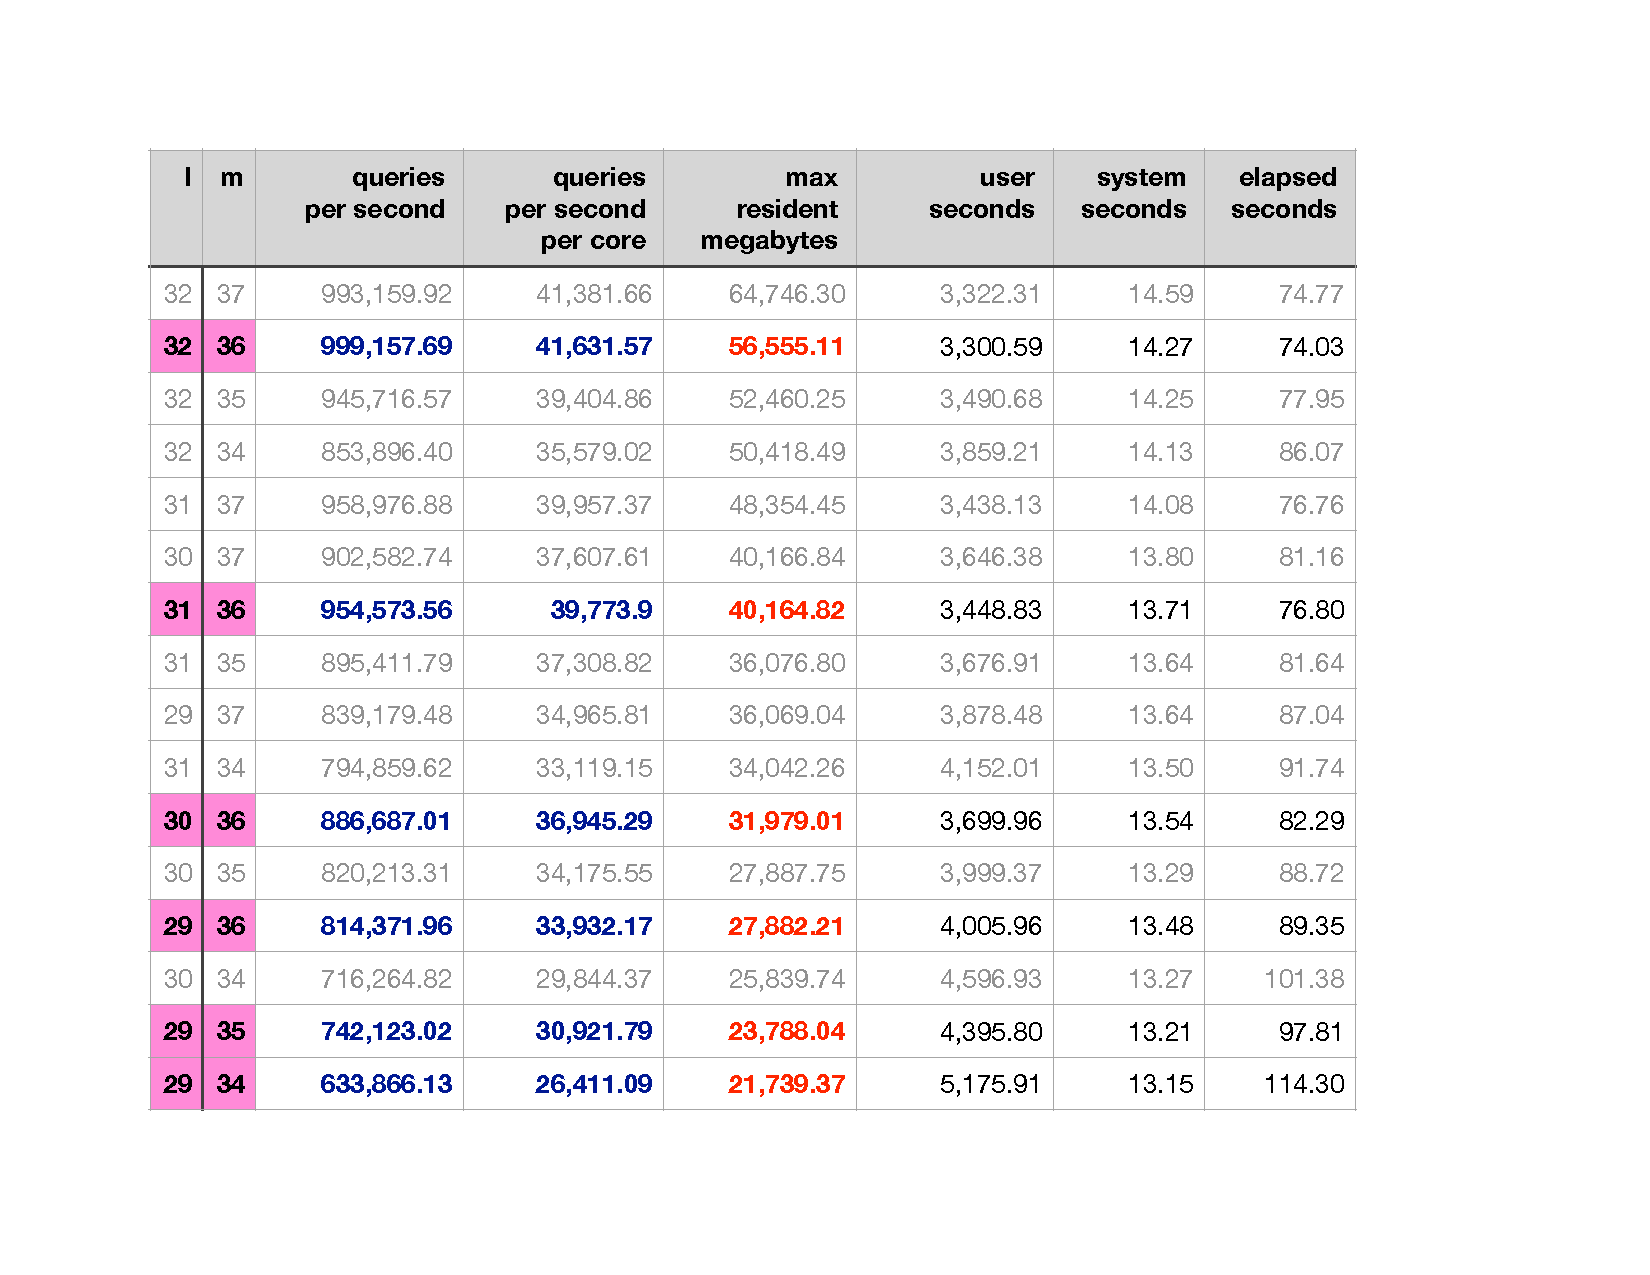
\includegraphics[width=1.4\textwidth]{awsslew-essential.pdf}
  }
}
\vskip -0.25in
We tried many combinations of index and bloom filter sizes (command line parameters \texttt{-l} and \texttt{-m}) to characterize the configuration that yields maximum performance as a function of memory footprint on our server test machine.

The highlighted values for \texttt{-l} and \texttt{-m} win over the greyed-out values by providing the same or better performance with smaller memory footprint.

The 8 measurements averaged to each value in this table are plotted separately on figure "Query Speed vs Memory Use".

\pagebreak
\subsection{Laptop Parameter Sweeps}


\hskip-0.75in\makebox[0pt][l]{
  \raisebox{-\totalheight-7em}[0pt][0pt]{
      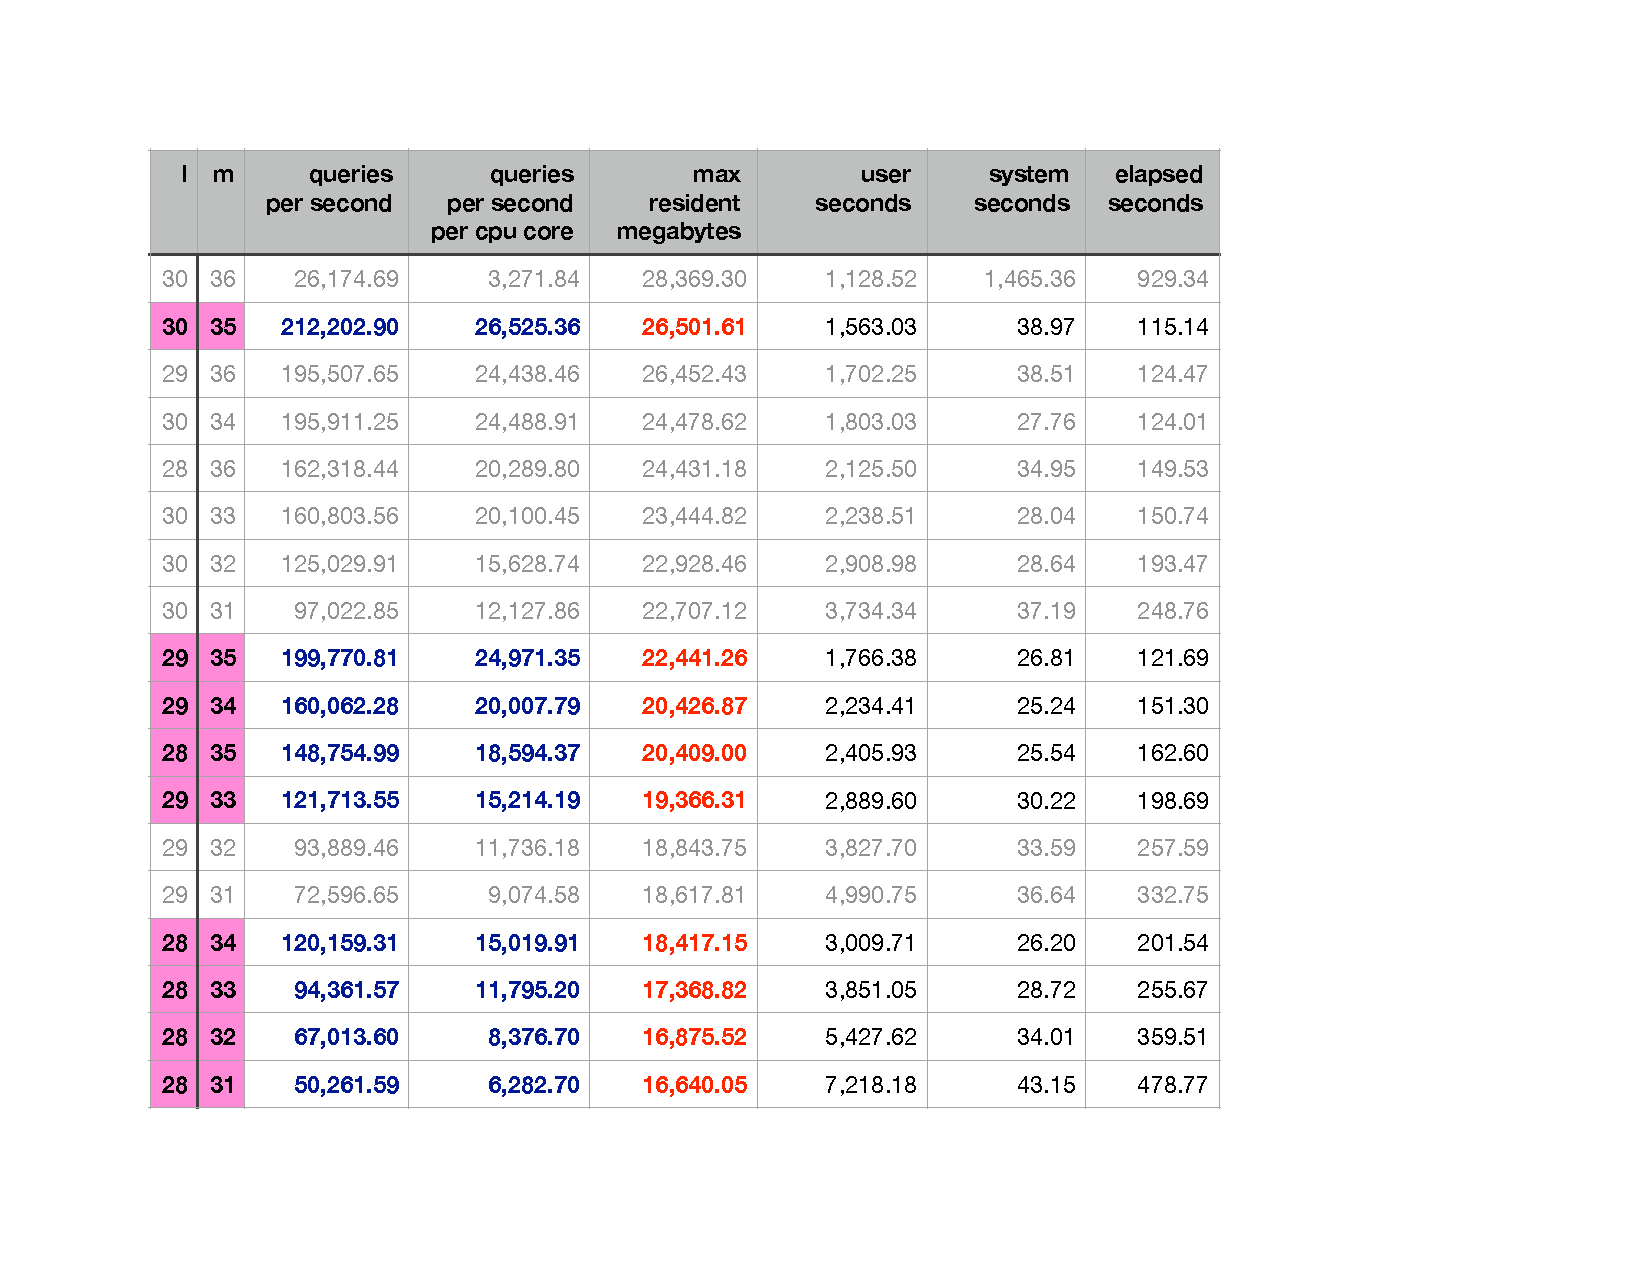
\includegraphics[width=1.55\textwidth]{laptop-essential.pdf}
  }
}
\vskip -0.25in
We tried many combinations of index and bloom filter sizes (command line parameters \texttt{-l} and \texttt{-m}) to characterize the configuration that yields maximum performance as a function of memory footprint on our laptop test machine.

The highlighted values for \texttt{-l} and \texttt{-m} win over the greyed-out values by providing the same or better performance with smaller memory footprint.

The 8 measurements averaged to each value in this table are plotted separately on figure "Query Speed vs Memory Use".

\pagebreak
\subsection{Query Speed Vs Memory Footprint}


\hskip-3em\makebox[0pt][l]{
  \raisebox{-\totalheight-8em}[0pt][0pt]{
      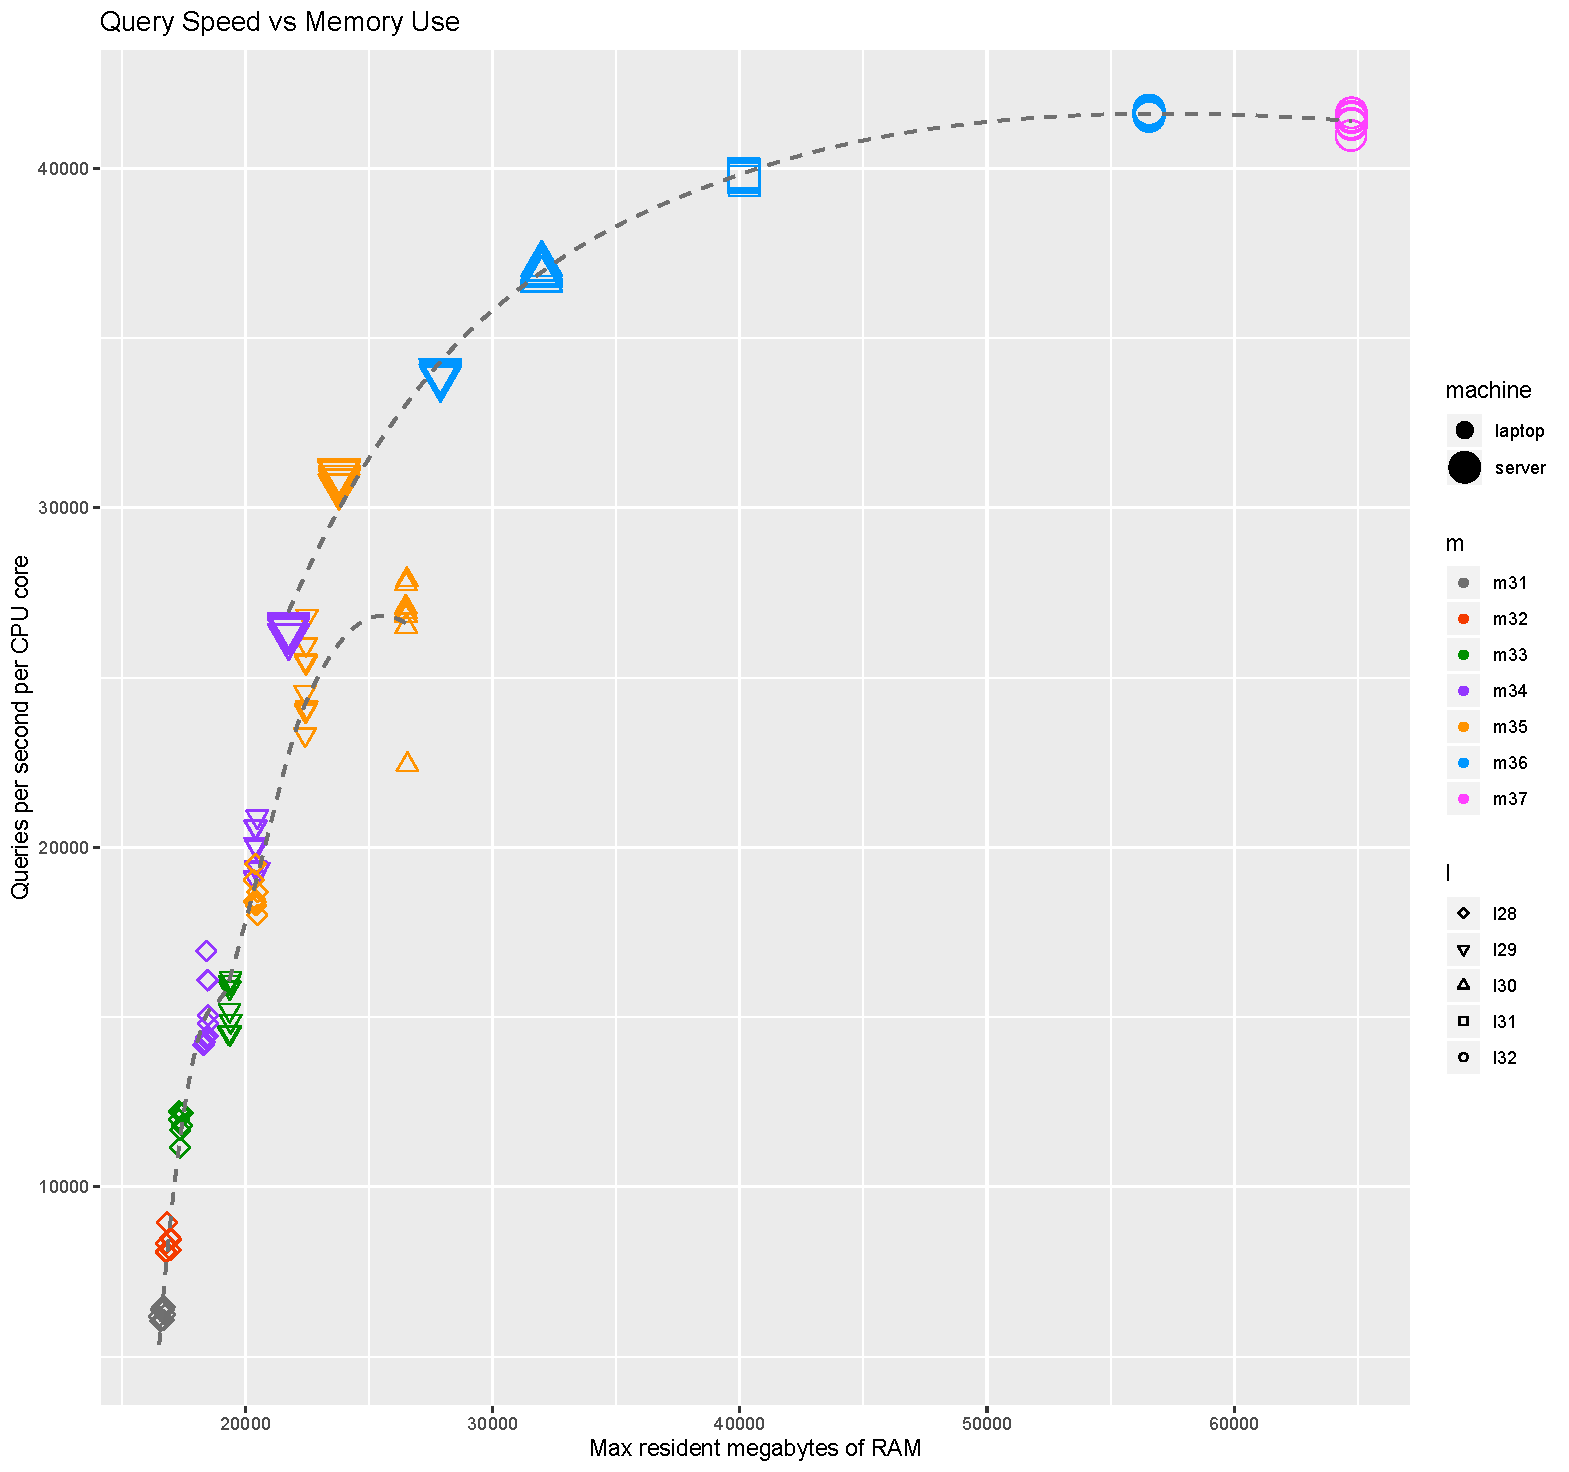
\includegraphics[width=1.2\textwidth]{speedvsmem.pdf}
  }
}
\vskip -0.25in

The winning \texttt{-l} and \texttt{-m} parameter configs from our server and laptop parameter sweeps were plotted to portray the relationship of performance to memory use.

Each config ran 8 times.  The server environment has low variance, so most server measurements overlap.  The laptop environment is very noisy, and one of the \texttt{-l 30} \texttt{-m 35} laptop measurements is an outlier bounded by I/O.

\pagebreak
\subsection{Server specs}


Machine:
\begin{itemize}
\item AWS r5.12xlarge.
\item 24 physical CPU cores (48 vCPU).
\item Intel 8175M CPU @ 2.50GHz.
\item Sustained all core Turbo CPU clock speed of up to 3.1 GHz.
\item 384 GB RAM
\item EBS gp2 RAID array providing 780 MB/sec bandwidth.
\end{itemize}

Operating system:
\begin{itemize}
\item Ubuntu 7.4.0 -- 18.04.01.
\end{itemize}

Compiler: 
\begin{itemize}
\item G++ 7.4.0.
\end{itemize}

\begin{alltt}
\footnotesize
> \textbf{\textcolor{brown}{g++ --version}}
g++ (Ubuntu 7.4.0-1ubuntu1~18.04.1) 7.4.0
Copyright (C) 2017 Free Software Foundation, Inc.
This is free software; see the source for copying conditions.  There is NO
warranty; not even for MERCHANTABILITY or FITNESS FOR A PARTICULAR PURPOSE.


> \textbf{\textcolor{brown}{lscpu}}
Architecture:        x86_64
CPU op-mode(s):      32-bit, 64-bit
Byte Order:          Little Endian
CPU(s):              48
On-line CPU(s) list: 0-47
Thread(s) per core:  2
Core(s) per socket:  24
Socket(s):           1
NUMA node(s):        1
Vendor ID:           GenuineIntel
CPU family:          6
Model:               85
Model name:          Intel(R) Xeon(R) Platinum 8175M CPU @ 2.50GHz
Stepping:            4
CPU MHz:             1341.926
BogoMIPS:            5000.00
Hypervisor vendor:   KVM
Virtualization type: full
L1d cache:           32K
L1i cache:           32K
L2 cache:            1024K
L3 cache:            33792K
NUMA node0 CPU(s):   0-47
Flags:               fpu vme de pse tsc msr pae mce cx8 apic sep mtrr pge mca cmov pat pse36
clflush mmx fxsr sse sse2 ss ht syscall nx pdpe1gb rdtscp lm constant_tsc arch_perfmon rep_good
nopl xtopology nonstop_tsc cpuid aperfmperf tsc_known_freq pni pclmulqdq monitor ssse3 fma cx16
pcid sse4_1 sse4_2 x2apic movbe popcnt tsc_deadline_timer aes xsave avx f16c rdrand hypervisor
lahf_lm abm 3dnowprefetch invpcid_single pti fsgsbase tsc_adjust bmi1 hle avx2 smep bmi2 erms
invpcid rtm mpx avx512f avx512dq rdseed adx smap clflushopt clwb avx512cd avx512bw avx512vl
xsaveopt xsavec xgetbv1 xsaves ida arat pku ospke
\end{alltt}

\subsection{Laptop specs}


Machine:
\begin{itemize}
\item Apple MacBook Pro (15-inch, 2019)
\item 8 physical CPU cores (16 vCPU).
\item Intel(R) Core(TM) i9-9980HK CPU @ 2.40GHz
\item Max Turbo CPU clock speed of up to 5.0 GHz.
\item 32 GB 2400 MHz DDR4 RAM.
\item 2TB APPLE SSD AP2048M
\end{itemize}

Operating system:
\begin{itemize}
\item Mac OS X 10.14.6
\end{itemize}

Compiler: 
\begin{itemize}
\item Apple LLVM version 10.0.1 (clang-1001.0.46.4)
\end{itemize}

\begin{alltt}
\footnotesize
> \textbf{\textcolor{brown}{g++ --version}}
Configured with: --prefix=/Applications/Xcode.app/Contents/Developer/usr
                 --with-gxx-include-dir=/usr/include/c++/4.2.1
Apple LLVM version 10.0.1 (clang-1001.0.46.4)
Target: x86_64-apple-darwin18.7.0
Thread model: posix
InstalledDir: /Applications/Xcode.app/Contents/Developer/Toolchains/XcodeDefault.xctoolchain/usr/bin

> \textbf{\textcolor{brown}{sysctl -n machdep.cpu.brand_string}}                                                                                                                                                 
Intel(R) Core(TM) i9-9980HK CPU @ 2.40GHz
\end{alltt}

\end{document}
